\documentclass[1p]{elsarticle_modified}
%\bibliographystyle{elsarticle-num}

%\usepackage[colorlinks]{hyperref}
%\usepackage{abbrmath_seonhwa} %\Abb, \Ascr, \Acal ,\Abf, \Afrak
\usepackage{amsfonts}
\usepackage{amssymb}
\usepackage{amsmath}
\usepackage{amsthm}
\usepackage{scalefnt}
\usepackage{amsbsy}
\usepackage{kotex}
\usepackage{caption}
\usepackage{subfig}
\usepackage{color}
\usepackage{graphicx}
\usepackage{xcolor} %% white, black, red, green, blue, cyan, magenta, yellow
\usepackage{float}
\usepackage{setspace}
\usepackage{hyperref}

\usepackage{tikz}
\usetikzlibrary{arrows}

\usepackage{multirow}
\usepackage{array} % fixed length table
\usepackage{hhline}

%%%%%%%%%%%%%%%%%%%%%
\makeatletter
\renewcommand*\env@matrix[1][\arraystretch]{%
	\edef\arraystretch{#1}%
	\hskip -\arraycolsep
	\let\@ifnextchar\new@ifnextchar
	\array{*\c@MaxMatrixCols c}}
\makeatother %https://tex.stackexchange.com/questions/14071/how-can-i-increase-the-line-spacing-in-a-matrix
%%%%%%%%%%%%%%%

\usepackage[normalem]{ulem}

\newcommand{\msout}[1]{\ifmmode\text{\sout{\ensuremath{#1}}}\else\sout{#1}\fi}
%SOURCE: \msout is \stkout macro in https://tex.stackexchange.com/questions/20609/strikeout-in-math-mode

\newcommand{\cancel}[1]{
	\ifmmode
	{\color{red}\msout{#1}}
	\else
	{\color{red}\sout{#1}}
	\fi
}

\newcommand{\add}[1]{
	{\color{blue}\uwave{#1}}
}

\newcommand{\replace}[2]{
	\ifmmode
	{\color{red}\msout{#1}}{\color{blue}\uwave{#2}}
	\else
	{\color{red}\sout{#1}}{\color{blue}\uwave{#2}}
	\fi
}

\newcommand{\Sol}{\mathcal{S}} %segment
\newcommand{\D}{D} %diagram
\newcommand{\A}{\mathcal{A}} %arc


%%%%%%%%%%%%%%%%%%%%%%%%%%%%%5 test

\def\sl{\operatorname{\textup{SL}}(2,\Cbb)}
\def\psl{\operatorname{\textup{PSL}}(2,\Cbb)}
\def\quan{\mkern 1mu \triangleright \mkern 1mu}

\theoremstyle{definition}
\newtheorem{thm}{Theorem}[section]
\newtheorem{prop}[thm]{Proposition}
\newtheorem{lem}[thm]{Lemma}
\newtheorem{ques}[thm]{Question}
\newtheorem{cor}[thm]{Corollary}
\newtheorem{defn}[thm]{Definition}
\newtheorem{exam}[thm]{Example}
\newtheorem{rmk}[thm]{Remark}
\newtheorem{alg}[thm]{Algorithm}

\newcommand{\I}{\sqrt{-1}}
\begin{document}

%\begin{frontmatter}
%
%\title{Boundary parabolic representations of knots up to 8 crossings}
%
%%% Group authors per affiliation:
%\author{Yunhi Cho} 
%\address{Department of Mathematics, University of Seoul, Seoul, Korea}
%\ead{yhcho@uos.ac.kr}
%
%
%\author{Seonhwa Kim} %\fnref{s_kim}}
%\address{Center for Geometry and Physics, Institute for Basic Science, Pohang, 37673, Korea}
%\ead{ryeona17@ibs.re.kr}
%
%\author{Hyuk Kim}
%\address{Department of Mathematical Sciences, Seoul National University, Seoul 08826, Korea}
%\ead{hyukkim@snu.ac.kr}
%
%\author{Seokbeom Yoon}
%\address{Department of Mathematical Sciences, Seoul National University, Seoul, 08826,  Korea}
%\ead{sbyoon15@snu.ac.kr}
%
%\begin{abstract}
%We find all boundary parabolic representation of knots up to 8 crossings.
%
%\end{abstract}
%\begin{keyword}
%    \MSC[2010] 57M25 
%\end{keyword}
%
%\end{frontmatter}

%\linenumbers
%\tableofcontents
%
\newcommand\colored[1]{\textcolor{white}{\rule[-0.35ex]{0.8em}{1.4ex}}\kern-0.8em\color{red} #1}%
%\newcommand\colored[1]{\textcolor{white}{ #1}\kern-2.17ex	\textcolor{white}{ #1}\kern-1.81ex	\textcolor{white}{ #1}\kern-2.15ex\color{red}#1	}

{\Large $\underline{12a_{0371}~(K12a_{0371})}$}

\setlength{\tabcolsep}{10pt}
\renewcommand{\arraystretch}{1.6}
\vspace{1cm}\begin{tabular}{m{100pt}>{\centering\arraybackslash}m{274pt}}
\multirow{5}{120pt}{
	\centering
	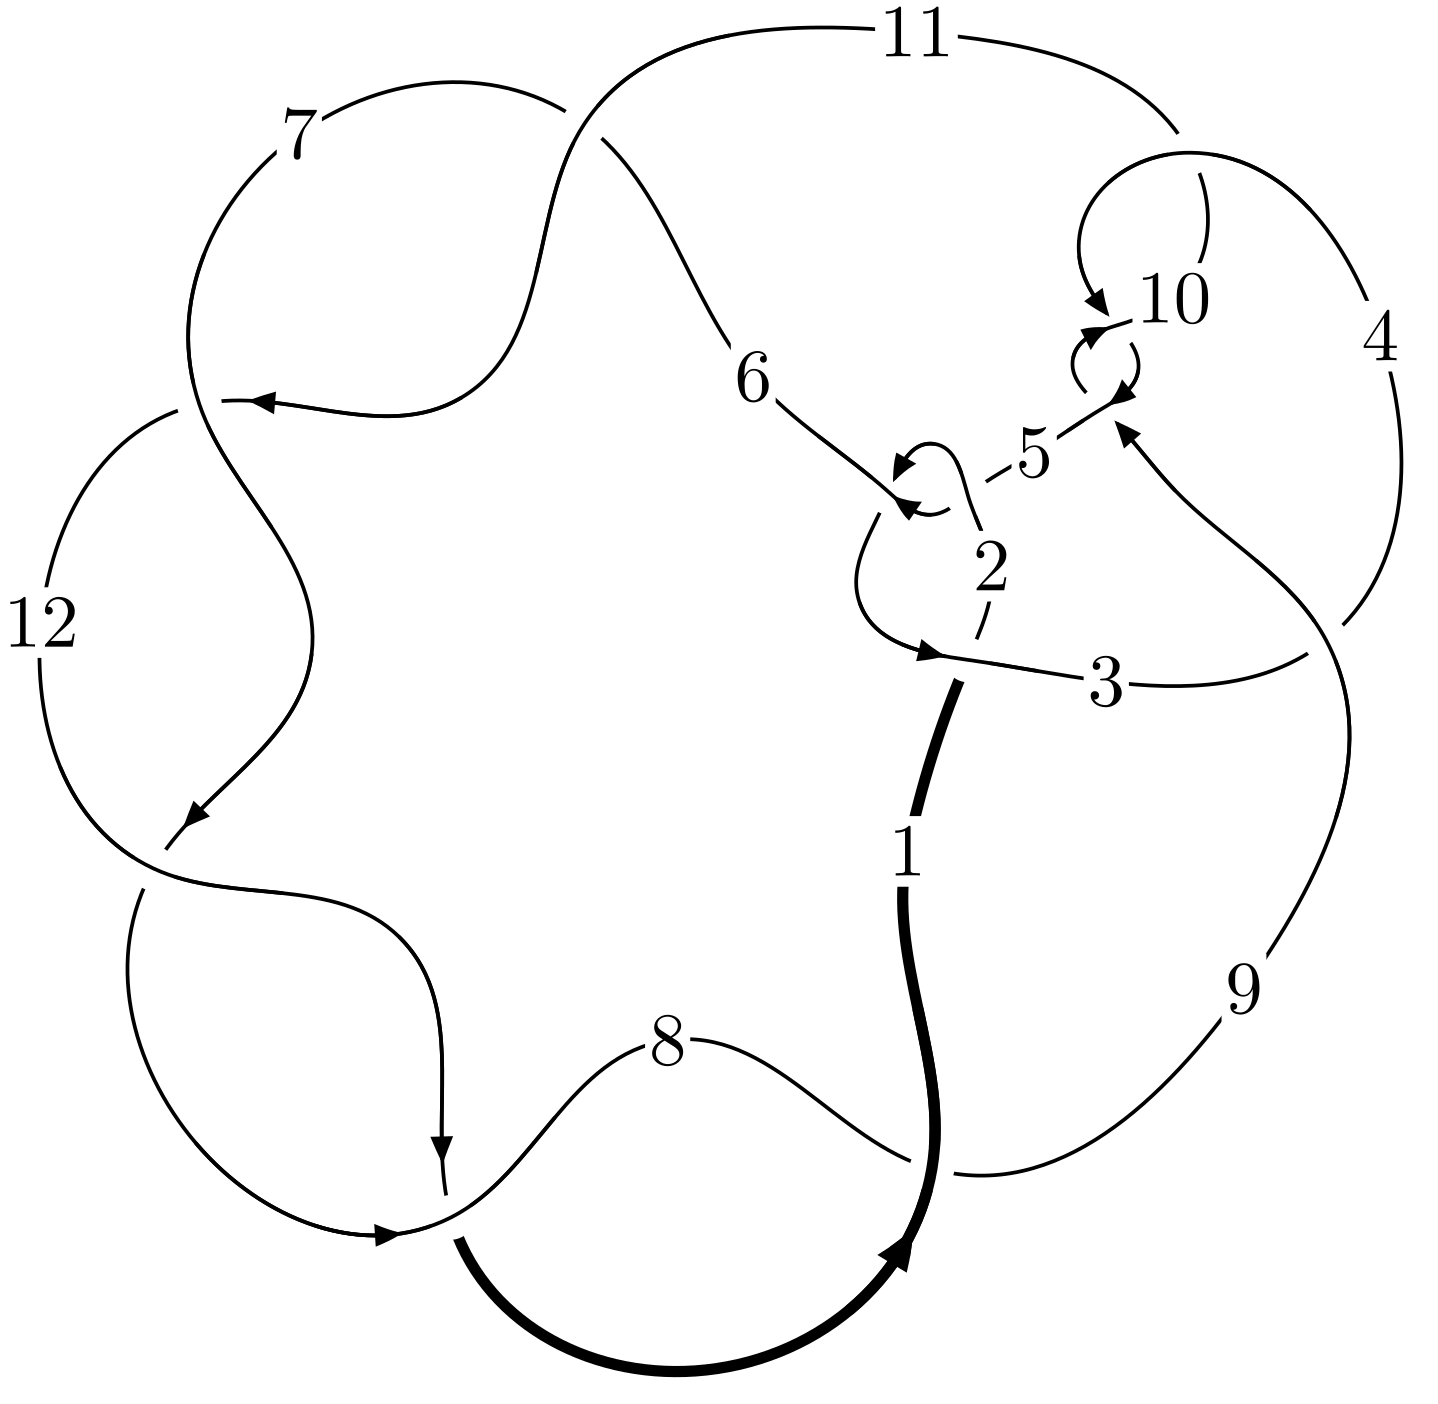
\includegraphics[width=112pt]{../../../GIT/diagram.site/Diagrams/png/1172_12a_0371.png}\\
\ \ \ A knot diagram\footnotemark}&
\allowdisplaybreaks
\textbf{Linearized knot diagam} \\
\cline{2-2}
 &
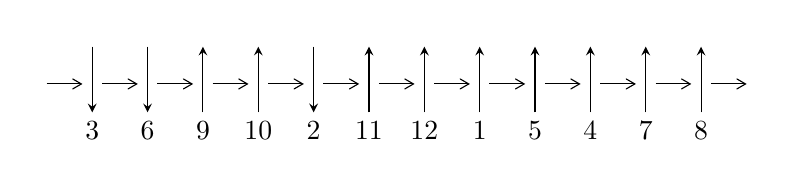
\begin{tikzpicture}[x=20pt, y=17pt]
	% nodes
	\node (C0) at (0, 0) {};
	\node (C1) at (1, 0) {};
	\node (C1U) at (1, +1) {};
	\node (C1D) at (1, -1) {3};

	\node (C2) at (2, 0) {};
	\node (C2U) at (2, +1) {};
	\node (C2D) at (2, -1) {6};

	\node (C3) at (3, 0) {};
	\node (C3U) at (3, +1) {};
	\node (C3D) at (3, -1) {9};

	\node (C4) at (4, 0) {};
	\node (C4U) at (4, +1) {};
	\node (C4D) at (4, -1) {10};

	\node (C5) at (5, 0) {};
	\node (C5U) at (5, +1) {};
	\node (C5D) at (5, -1) {2};

	\node (C6) at (6, 0) {};
	\node (C6U) at (6, +1) {};
	\node (C6D) at (6, -1) {11};

	\node (C7) at (7, 0) {};
	\node (C7U) at (7, +1) {};
	\node (C7D) at (7, -1) {12};

	\node (C8) at (8, 0) {};
	\node (C8U) at (8, +1) {};
	\node (C8D) at (8, -1) {1};

	\node (C9) at (9, 0) {};
	\node (C9U) at (9, +1) {};
	\node (C9D) at (9, -1) {5};

	\node (C10) at (10, 0) {};
	\node (C10U) at (10, +1) {};
	\node (C10D) at (10, -1) {4};

	\node (C11) at (11, 0) {};
	\node (C11U) at (11, +1) {};
	\node (C11D) at (11, -1) {7};

	\node (C12) at (12, 0) {};
	\node (C12U) at (12, +1) {};
	\node (C12D) at (12, -1) {8};
	\node (C13) at (13, 0) {};

	% arrows
	\draw[->,>={angle 60}]
	(C0) edge (C1) (C1) edge (C2) (C2) edge (C3) (C3) edge (C4) (C4) edge (C5) (C5) edge (C6) (C6) edge (C7) (C7) edge (C8) (C8) edge (C9) (C9) edge (C10) (C10) edge (C11) (C11) edge (C12) (C12) edge (C13) ;	\draw[->,>=stealth]
	(C1U) edge (C1D) (C2U) edge (C2D) (C3D) edge (C3U) (C4D) edge (C4U) (C5U) edge (C5D) (C6D) edge (C6U) (C7D) edge (C7U) (C8D) edge (C8U) (C9D) edge (C9U) (C10D) edge (C10U) (C11D) edge (C11U) (C12D) edge (C12U) ;
	\end{tikzpicture} \\
\hhline{~~} \\& 
\textbf{Solving Sequence} \\ \cline{2-2} 
 &
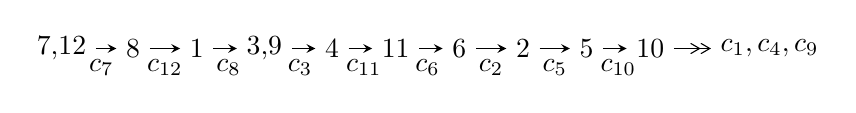
\begin{tikzpicture}[x=23pt, y=7pt]
	% node
	\node (A0) at (-1/8, 0) {7,12};
	\node (A1) at (1, 0) {8};
	\node (A2) at (2, 0) {1};
	\node (A3) at (49/16, 0) {3,9};
	\node (A4) at (33/8, 0) {4};
	\node (A5) at (41/8, 0) {11};
	\node (A6) at (49/8, 0) {6};
	\node (A7) at (57/8, 0) {2};
	\node (A8) at (65/8, 0) {5};
	\node (A9) at (73/8, 0) {10};
	\node (C1) at (1/2, -1) {$c_{7}$};
	\node (C2) at (3/2, -1) {$c_{12}$};
	\node (C3) at (5/2, -1) {$c_{8}$};
	\node (C4) at (29/8, -1) {$c_{3}$};
	\node (C5) at (37/8, -1) {$c_{11}$};
	\node (C6) at (45/8, -1) {$c_{6}$};
	\node (C7) at (53/8, -1) {$c_{2}$};
	\node (C8) at (61/8, -1) {$c_{5}$};
	\node (C9) at (69/8, -1) {$c_{10}$};
	\node (A10) at (11, 0) {$c_{1},c_{4},c_{9}$};

	% edge
	\draw[->,>=stealth]	
	(A0) edge (A1) (A1) edge (A2) (A2) edge (A3) (A3) edge (A4) (A4) edge (A5) (A5) edge (A6) (A6) edge (A7) (A7) edge (A8) (A8) edge (A9) ;
	\draw[->>,>={angle 60}]	
	(A9) edge (A10);
\end{tikzpicture} \\ 

\end{tabular} \\

\footnotetext{
The image of knot diagram is generated by the software ``\textbf{Draw programme}" developed by Andrew Bartholomew(\url{http://www.layer8.co.uk/maths/draw/index.htm\#Running-draw}), where we modified some parts for our purpose(\url{https://github.com/CATsTAILs/LinksPainter}).
}\phantom \\ \newline 
\centering \textbf{Ideals for irreducible components\footnotemark of $X_{\text{par}}$} 
 
\begin{align*}
I^u_{1}&=\langle 
6.22403\times10^{15} u^{53}-2.16644\times10^{16} u^{52}+\cdots+1.15315\times10^{16} b+1.86130\times10^{15},\\
\phantom{I^u_{1}}&\phantom{= \langle  }-3.84141\times10^{15} u^{53}-5.38285\times10^{15} u^{52}+\cdots+3.45944\times10^{16} a+4.72334\times10^{16},\;u^{54}-2 u^{53}+\cdots-9 u+3\rangle \\
I^u_{2}&=\langle 
b+1,\;a-1,\;u^2- u-1\rangle \\
I^u_{3}&=\langle 
- a u+b- u-1,\;a^2+2 a+3,\;u^2+u-1\rangle \\
\\
\end{align*}
\raggedright * 3 irreducible components of $\dim_{\mathbb{C}}=0$, with total 60 representations.\\
\footnotetext{All coefficients of polynomials are rational numbers. But the coefficients are sometimes approximated in decimal forms when there is not enough margin.}
\newpage
\renewcommand{\arraystretch}{1}
\centering \section*{I. $I^u_{1}= \langle 6.22\times10^{15} u^{53}-2.17\times10^{16} u^{52}+\cdots+1.15\times10^{16} b+1.86\times10^{15},\;-3.84\times10^{15} u^{53}-5.38\times10^{15} u^{52}+\cdots+3.46\times10^{16} a+4.72\times10^{16},\;u^{54}-2 u^{53}+\cdots-9 u+3 \rangle$}
\flushleft \textbf{(i) Arc colorings}\\
\begin{tabular}{m{7pt} m{180pt} m{7pt} m{180pt} }
\flushright $a_{7}=$&$\begin{pmatrix}1\\0\end{pmatrix}$ \\
\flushright $a_{12}=$&$\begin{pmatrix}0\\u\end{pmatrix}$ \\
\flushright $a_{8}=$&$\begin{pmatrix}1\\- u^2\end{pmatrix}$ \\
\flushright $a_{1}=$&$\begin{pmatrix}u\\- u^3+u\end{pmatrix}$ \\
\flushright $a_{3}=$&$\begin{pmatrix}0.111041 u^{53}+0.155599 u^{52}+\cdots+4.11220 u-1.36535\\-0.539742 u^{53}+1.87871 u^{52}+\cdots+3.32643 u-0.161411\end{pmatrix}$ \\
\flushright $a_{9}=$&$\begin{pmatrix}- u^2+1\\u^4-2 u^2\end{pmatrix}$ \\
\flushright $a_{4}=$&$\begin{pmatrix}0.607017 u^{53}+0.0379752 u^{52}+\cdots+3.56687 u-1.29746\\-1.30686 u^{53}+2.07232 u^{52}+\cdots-0.567204 u+1.29954\end{pmatrix}$ \\
\flushright $a_{11}=$&$\begin{pmatrix}- u\\u\end{pmatrix}$ \\
\flushright $a_{6}=$&$\begin{pmatrix}- u^2+1\\u^2\end{pmatrix}$ \\
\flushright $a_{2}=$&$\begin{pmatrix}0.874650 u^{53}+0.540026 u^{52}+\cdots+6.16049 u-2.08423\\-1.85817 u^{53}+1.24119 u^{52}+\cdots-7.27374 u+3.92680\end{pmatrix}$ \\
\flushright $a_{5}=$&$\begin{pmatrix}0.818828 u^{53}-1.31508 u^{52}+\cdots-12.3614 u+1.51037\\-1.22880 u^{53}+1.80213 u^{52}+\cdots+3.71901 u-0.853328\end{pmatrix}$ \\
\flushright $a_{10}=$&$\begin{pmatrix}-0.287418 u^{53}-0.715155 u^{52}+\cdots-7.57410 u+3.47537\\0.496261 u^{53}+1.55979 u^{52}+\cdots+11.6363 u-3.00772\end{pmatrix}$\\&\end{tabular}
\flushleft \textbf{(ii) Obstruction class $= -1$}\\~\\
\flushleft \textbf{(iii) Cusp Shapes $= -\frac{1362927332552725}{5765740254433699} u^{53}-\frac{23381515261364111}{5765740254433699} u^{52}+\cdots-\frac{315387112075661492}{5765740254433699} u+\frac{81812943695667795}{5765740254433699}$}\\~\\
\newpage\renewcommand{\arraystretch}{1}
\flushleft \textbf{(iv) u-Polynomials at the component}\newline \\
\begin{tabular}{m{50pt}|m{274pt}}
Crossings & \hspace{64pt}u-Polynomials at each crossing \\
\hline $$\begin{aligned}c_{1}\end{aligned}$$&$\begin{aligned}
&u^{54}+25 u^{53}+\cdots+4038 u+121
\end{aligned}$\\
\hline $$\begin{aligned}c_{2},c_{5}\end{aligned}$$&$\begin{aligned}
&u^{54}+3 u^{53}+\cdots-12 u+11
\end{aligned}$\\
\hline $$\begin{aligned}c_{3}\end{aligned}$$&$\begin{aligned}
&u^{54}- u^{53}+\cdots-1064 u+212
\end{aligned}$\\
\hline $$\begin{aligned}c_{4},c_{9},c_{10}\end{aligned}$$&$\begin{aligned}
&u^{54}+u^{53}+\cdots-36 u^2+4
\end{aligned}$\\
\hline $$\begin{aligned}c_{6},c_{7},c_{8}\\c_{11},c_{12}\end{aligned}$$&$\begin{aligned}
&u^{54}+2 u^{53}+\cdots+9 u+3
\end{aligned}$\\
\hline
\end{tabular}\\~\\
\newpage\renewcommand{\arraystretch}{1}
\flushleft \textbf{(v) Riley Polynomials at the component}\newline \\
\begin{tabular}{m{50pt}|m{274pt}}
Crossings & \hspace{64pt}Riley Polynomials at each crossing \\
\hline $$\begin{aligned}c_{1}\end{aligned}$$&$\begin{aligned}
&y^{54}+15 y^{53}+\cdots-5943246 y+14641
\end{aligned}$\\
\hline $$\begin{aligned}c_{2},c_{5}\end{aligned}$$&$\begin{aligned}
&y^{54}-25 y^{53}+\cdots-4038 y+121
\end{aligned}$\\
\hline $$\begin{aligned}c_{3}\end{aligned}$$&$\begin{aligned}
&y^{54}-11 y^{53}+\cdots-679264 y+44944
\end{aligned}$\\
\hline $$\begin{aligned}c_{4},c_{9},c_{10}\end{aligned}$$&$\begin{aligned}
&y^{54}+49 y^{53}+\cdots-288 y+16
\end{aligned}$\\
\hline $$\begin{aligned}c_{6},c_{7},c_{8}\\c_{11},c_{12}\end{aligned}$$&$\begin{aligned}
&y^{54}-72 y^{53}+\cdots+15 y+9
\end{aligned}$\\
\hline
\end{tabular}\\~\\
\newpage\flushleft \textbf{(vi) Complex Volumes and Cusp Shapes}
$$\begin{array}{c|c|c}  
\text{Solutions to }I^u_{1}& \I (\text{vol} + \sqrt{-1}CS) & \text{Cusp shape}\\
 \hline 
\begin{aligned}
u &= -1.033200 + 0.205031 I \\
a &= -0.154928 - 0.608627 I \\
b &= \phantom{-}0.043531 - 1.156360 I\end{aligned}
 & \phantom{-}2.48098 - 2.65644 I & \phantom{-0.000000 } 0 \\ \hline\begin{aligned}
u &= -1.033200 - 0.205031 I \\
a &= -0.154928 + 0.608627 I \\
b &= \phantom{-}0.043531 + 1.156360 I\end{aligned}
 & \phantom{-}2.48098 + 2.65644 I & \phantom{-0.000000 } 0 \\ \hline\begin{aligned}
u &= -0.909027 + 0.201496 I \\
a &= \phantom{-}1.133080 - 0.239512 I \\
b &= -1.44506 + 0.44518 I\end{aligned}
 & -4.31420 - 2.29321 I & \phantom{-}6.00000 + 3.97838 I \\ \hline\begin{aligned}
u &= -0.909027 - 0.201496 I \\
a &= \phantom{-}1.133080 + 0.239512 I \\
b &= -1.44506 - 0.44518 I\end{aligned}
 & -4.31420 + 2.29321 I & \phantom{-}6.00000 - 3.97838 I \\ \hline\begin{aligned}
u &= -1.002340 + 0.391017 I \\
a &= \phantom{-}0.373522 - 0.490684 I \\
b &= \phantom{-}0.159427 - 1.337780 I\end{aligned}
 & -0.92608 - 10.90870 I & \phantom{-0.000000 } 0 \\ \hline\begin{aligned}
u &= -1.002340 - 0.391017 I \\
a &= \phantom{-}0.373522 + 0.490684 I \\
b &= \phantom{-}0.159427 + 1.337780 I\end{aligned}
 & -0.92608 + 10.90870 I & \phantom{-0.000000 } 0 \\ \hline\begin{aligned}
u &= -1.035390 + 0.306908 I \\
a &= -0.826876 + 0.402579 I \\
b &= \phantom{-}0.073409 + 0.249362 I\end{aligned}
 & \phantom{-}1.28679 - 5.35006 I & \phantom{-0.000000 } 0 \\ \hline\begin{aligned}
u &= -1.035390 - 0.306908 I \\
a &= -0.826876 - 0.402579 I \\
b &= \phantom{-}0.073409 - 0.249362 I\end{aligned}
 & \phantom{-}1.28679 + 5.35006 I & \phantom{-0.000000 } 0 \\ \hline\begin{aligned}
u &= \phantom{-}1.035020 + 0.327197 I \\
a &= -0.175793 - 0.504243 I \\
b &= -0.136856 - 1.285110 I\end{aligned}
 & \phantom{-}4.34470 + 6.91339 I & \phantom{-0.000000 } 0 \\ \hline\begin{aligned}
u &= \phantom{-}1.035020 - 0.327197 I \\
a &= -0.175793 + 0.504243 I \\
b &= -0.136856 + 1.285110 I\end{aligned}
 & \phantom{-}4.34470 - 6.91339 I & \phantom{-0.000000 } 0\\
 \hline 
 \end{array}$$\newpage$$\begin{array}{c|c|c}  
\text{Solutions to }I^u_{1}& \I (\text{vol} + \sqrt{-1}CS) & \text{Cusp shape}\\
 \hline 
\begin{aligned}
u &= \phantom{-}1.084440 + 0.195251 I \\
a &= \phantom{-}0.775059 + 0.381941 I \\
b &= -0.098656 + 0.410716 I\end{aligned}
 & \phantom{-}5.85353 + 1.52576 I & \phantom{-0.000000 } 0 \\ \hline\begin{aligned}
u &= \phantom{-}1.084440 - 0.195251 I \\
a &= \phantom{-}0.775059 - 0.381941 I \\
b &= -0.098656 - 0.410716 I\end{aligned}
 & \phantom{-}5.85353 - 1.52576 I & \phantom{-0.000000 } 0 \\ \hline\begin{aligned}
u &= -1.120580 + 0.004894 I \\
a &= -0.589724 + 0.389273 I \\
b &= \phantom{-}0.128535 + 0.742200 I\end{aligned}
 & \phantom{-}3.05827 + 2.30358 I & \phantom{-0.000000 } 0 \\ \hline\begin{aligned}
u &= -1.120580 - 0.004894 I \\
a &= -0.589724 - 0.389273 I \\
b &= \phantom{-}0.128535 - 0.742200 I\end{aligned}
 & \phantom{-}3.05827 - 2.30358 I & \phantom{-0.000000 } 0 \\ \hline\begin{aligned}
u &= \phantom{-}0.849728 + 0.155769 I \\
a &= \phantom{-}0.39360 - 1.41513 I \\
b &= \phantom{-}0.39372 - 1.40393 I\end{aligned}
 & -4.89459 + 1.45597 I & \phantom{-}7.23813 - 5.57336 I \\ \hline\begin{aligned}
u &= \phantom{-}0.849728 - 0.155769 I \\
a &= \phantom{-}0.39360 + 1.41513 I \\
b &= \phantom{-}0.39372 + 1.40393 I\end{aligned}
 & -4.89459 - 1.45597 I & \phantom{-}7.23813 + 5.57336 I \\ \hline\begin{aligned}
u &= \phantom{-}0.824308\phantom{ +0.000000I} \\
a &= -1.10776\phantom{ +0.000000I} \\
b &= \phantom{-}1.34525\phantom{ +0.000000I}\end{aligned}
 & -0.0557748\phantom{ +0.000000I} & \phantom{-}15.4170\phantom{ +0.000000I} \\ \hline\begin{aligned}
u &= \phantom{-}0.611997 + 0.492090 I \\
a &= -0.641324 - 0.317061 I \\
b &= \phantom{-}0.772587 + 0.690967 I\end{aligned}
 & -3.28887 - 3.64964 I & \phantom{-}5.12459 + 1.94620 I \\ \hline\begin{aligned}
u &= \phantom{-}0.611997 - 0.492090 I \\
a &= -0.641324 + 0.317061 I \\
b &= \phantom{-}0.772587 - 0.690967 I\end{aligned}
 & -3.28887 + 3.64964 I & \phantom{-}5.12459 - 1.94620 I \\ \hline\begin{aligned}
u &= \phantom{-}0.184324 + 0.638362 I \\
a &= \phantom{-}1.16880 + 1.08855 I \\
b &= \phantom{-}0.356445 - 0.466281 I\end{aligned}
 & -4.58312 + 7.42689 I & \phantom{-}2.31046 - 6.99724 I\\
 \hline 
 \end{array}$$\newpage$$\begin{array}{c|c|c}  
\text{Solutions to }I^u_{1}& \I (\text{vol} + \sqrt{-1}CS) & \text{Cusp shape}\\
 \hline 
\begin{aligned}
u &= \phantom{-}0.184324 - 0.638362 I \\
a &= \phantom{-}1.16880 - 1.08855 I \\
b &= \phantom{-}0.356445 + 0.466281 I\end{aligned}
 & -4.58312 - 7.42689 I & \phantom{-}2.31046 + 6.99724 I \\ \hline\begin{aligned}
u &= \phantom{-}0.454241 + 0.453212 I \\
a &= \phantom{-}0.661574 + 0.833835 I \\
b &= \phantom{-}0.301434 - 0.167958 I\end{aligned}
 & -2.14560 + 0.88769 I & \phantom{-}6.18591 - 4.35554 I \\ \hline\begin{aligned}
u &= \phantom{-}0.454241 - 0.453212 I \\
a &= \phantom{-}0.661574 - 0.833835 I \\
b &= \phantom{-}0.301434 + 0.167958 I\end{aligned}
 & -2.14560 - 0.88769 I & \phantom{-}6.18591 + 4.35554 I \\ \hline\begin{aligned}
u &= -0.455135 + 0.442932 I \\
a &= \phantom{-}0.490955 - 0.173110 I \\
b &= -0.587686 + 0.546971 I\end{aligned}
 & \phantom{-}1.046370 + 0.494844 I & \phantom{-}10.64023 + 0.18722 I \\ \hline\begin{aligned}
u &= -0.455135 - 0.442932 I \\
a &= \phantom{-}0.490955 + 0.173110 I \\
b &= -0.587686 - 0.546971 I\end{aligned}
 & \phantom{-}1.046370 - 0.494844 I & \phantom{-}10.64023 - 0.18722 I \\ \hline\begin{aligned}
u &= -0.248292 + 0.564754 I \\
a &= -0.98947 + 1.14172 I \\
b &= -0.374122 - 0.374831 I\end{aligned}
 & \phantom{-}0.36246 - 3.88016 I & \phantom{-}7.34275 + 7.06872 I \\ \hline\begin{aligned}
u &= -0.248292 - 0.564754 I \\
a &= -0.98947 - 1.14172 I \\
b &= -0.374122 + 0.374831 I\end{aligned}
 & \phantom{-}0.36246 + 3.88016 I & \phantom{-}7.34275 - 7.06872 I \\ \hline\begin{aligned}
u &= \phantom{-}0.260818 + 0.544636 I \\
a &= -0.240106 - 0.253128 I \\
b &= \phantom{-}0.306471 + 0.627052 I\end{aligned}
 & -2.73742 + 2.46050 I & \phantom{-}4.87493 - 3.38491 I \\ \hline\begin{aligned}
u &= \phantom{-}0.260818 - 0.544636 I \\
a &= -0.240106 + 0.253128 I \\
b &= \phantom{-}0.306471 - 0.627052 I\end{aligned}
 & -2.73742 - 2.46050 I & \phantom{-}4.87493 + 3.38491 I \\ \hline\begin{aligned}
u &= -1.54880 + 0.05145 I \\
a &= -0.928695 - 0.013670 I \\
b &= \phantom{-}0.951552 + 0.345464 I\end{aligned}
 & \phantom{-}3.71593 + 1.81884 I & \phantom{-0.000000 } 0\\
 \hline 
 \end{array}$$\newpage$$\begin{array}{c|c|c}  
\text{Solutions to }I^u_{1}& \I (\text{vol} + \sqrt{-1}CS) & \text{Cusp shape}\\
 \hline 
\begin{aligned}
u &= -1.54880 - 0.05145 I \\
a &= -0.928695 + 0.013670 I \\
b &= \phantom{-}0.951552 - 0.345464 I\end{aligned}
 & \phantom{-}3.71593 - 1.81884 I & \phantom{-0.000000 } 0 \\ \hline\begin{aligned}
u &= -0.421997\phantom{ +0.000000I} \\
a &= -0.252936\phantom{ +0.000000I} \\
b &= -0.323293\phantom{ +0.000000I}\end{aligned}
 & \phantom{-}0.611710\phantom{ +0.000000I} & \phantom{-}16.5140\phantom{ +0.000000I} \\ \hline\begin{aligned}
u &= \phantom{-}1.59012\phantom{ +0.000000I} \\
a &= \phantom{-}1.01605\phantom{ +0.000000I} \\
b &= -1.17062\phantom{ +0.000000I}\end{aligned}
 & \phantom{-}7.70118\phantom{ +0.000000I} & \phantom{-0.000000 } 0 \\ \hline\begin{aligned}
u &= \phantom{-}0.209460 + 0.318057 I \\
a &= \phantom{-}0.26966 + 1.81111 I \\
b &= \phantom{-}0.598382 - 0.217505 I\end{aligned}
 & -1.44891 + 0.87205 I & -0.45042 - 2.57700 I \\ \hline\begin{aligned}
u &= \phantom{-}0.209460 - 0.318057 I \\
a &= \phantom{-}0.26966 - 1.81111 I \\
b &= \phantom{-}0.598382 + 0.217505 I\end{aligned}
 & -1.44891 - 0.87205 I & -0.45042 + 2.57700 I \\ \hline\begin{aligned}
u &= \phantom{-}0.052280 + 0.369852 I \\
a &= -2.16277 + 2.09624 I \\
b &= -0.774037 - 0.521212 I\end{aligned}
 & -7.25657 + 0.32248 I & -3.59043 - 0.24507 I \\ \hline\begin{aligned}
u &= \phantom{-}0.052280 - 0.369852 I \\
a &= -2.16277 - 2.09624 I \\
b &= -0.774037 + 0.521212 I\end{aligned}
 & -7.25657 - 0.32248 I & -3.59043 + 0.24507 I \\ \hline\begin{aligned}
u &= -1.68847 + 0.03150 I \\
a &= -0.90904 - 3.14347 I \\
b &= \phantom{-}1.74981 + 5.17567 I\end{aligned}
 & \phantom{-}4.15513 - 2.12237 I & \phantom{-0.000000 } 0 \\ \hline\begin{aligned}
u &= -1.68847 - 0.03150 I \\
a &= -0.90904 + 3.14347 I \\
b &= \phantom{-}1.74981 - 5.17567 I\end{aligned}
 & \phantom{-}4.15513 + 2.12237 I & \phantom{-0.000000 } 0 \\ \hline\begin{aligned}
u &= -1.69091\phantom{ +0.000000I} \\
a &= -1.02001\phantom{ +0.000000I} \\
b &= \phantom{-}0.854840\phantom{ +0.000000I}\end{aligned}
 & \phantom{-}8.98922\phantom{ +0.000000I} & \phantom{-0.000000 } 0\\
 \hline 
 \end{array}$$\newpage$$\begin{array}{c|c|c}  
\text{Solutions to }I^u_{1}& \I (\text{vol} + \sqrt{-1}CS) & \text{Cusp shape}\\
 \hline 
\begin{aligned}
u &= \phantom{-}1.69828 + 0.04672 I \\
a &= \phantom{-}1.022170 + 0.018668 I \\
b &= -0.834861 + 0.045952 I\end{aligned}
 & \phantom{-}4.95768 + 3.23508 I & \phantom{-0.000000 } 0 \\ \hline\begin{aligned}
u &= \phantom{-}1.69828 - 0.04672 I \\
a &= \phantom{-}1.022170 - 0.018668 I \\
b &= -0.834861 - 0.045952 I\end{aligned}
 & \phantom{-}4.95768 - 3.23508 I & \phantom{-0.000000 } 0 \\ \hline\begin{aligned}
u &= \phantom{-}1.71944 + 0.10562 I \\
a &= -0.42831 - 2.69040 I \\
b &= \phantom{-}0.36112 + 4.43030 I\end{aligned}
 & \phantom{-}8.6699 + 12.9219 I & \phantom{-0.000000 } 0 \\ \hline\begin{aligned}
u &= \phantom{-}1.71944 - 0.10562 I \\
a &= -0.42831 + 2.69040 I \\
b &= \phantom{-}0.36112 - 4.43030 I\end{aligned}
 & \phantom{-}8.6699 - 12.9219 I & \phantom{-0.000000 } 0 \\ \hline\begin{aligned}
u &= \phantom{-}1.72963 + 0.05599 I \\
a &= \phantom{-}0.14187 - 2.61907 I \\
b &= -0.54631 + 4.33951 I\end{aligned}
 & \phantom{-}12.36250 + 3.74731 I & \phantom{-0.000000 } 0 \\ \hline\begin{aligned}
u &= \phantom{-}1.72963 - 0.05599 I \\
a &= \phantom{-}0.14187 + 2.61907 I \\
b &= -0.54631 - 4.33951 I\end{aligned}
 & \phantom{-}12.36250 - 3.74731 I & \phantom{-0.000000 } 0 \\ \hline\begin{aligned}
u &= \phantom{-}1.72946 + 0.07949 I \\
a &= \phantom{-}0.62410 + 1.44096 I \\
b &= -1.29088 - 2.56923 I\end{aligned}
 & \phantom{-}11.12150 + 6.92662 I & \phantom{-0.000000 } 0 \\ \hline\begin{aligned}
u &= \phantom{-}1.72946 - 0.07949 I \\
a &= \phantom{-}0.62410 - 1.44096 I \\
b &= -1.29088 + 2.56923 I\end{aligned}
 & \phantom{-}11.12150 - 6.92662 I & \phantom{-0.000000 } 0 \\ \hline\begin{aligned}
u &= -1.72986 + 0.08588 I \\
a &= \phantom{-}0.19966 - 2.64199 I \\
b &= \phantom{-}0.00573 + 4.36280 I\end{aligned}
 & \phantom{-}14.1686 - 8.6037 I & \phantom{-0.000000 } 0 \\ \hline\begin{aligned}
u &= -1.72986 - 0.08588 I \\
a &= \phantom{-}0.19966 + 2.64199 I \\
b &= \phantom{-}0.00573 - 4.36280 I\end{aligned}
 & \phantom{-}14.1686 + 8.6037 I & \phantom{-0.000000 } 0\\
 \hline 
 \end{array}$$\newpage$$\begin{array}{c|c|c}  
\text{Solutions to }I^u_{1}& \I (\text{vol} + \sqrt{-1}CS) & \text{Cusp shape}\\
 \hline 
\begin{aligned}
u &= -1.73989 + 0.05063 I \\
a &= -0.61741 + 1.65827 I \\
b &= \phantom{-}1.29019 - 2.88401 I\end{aligned}
 & \phantom{-}15.9719 - 2.5529 I & \phantom{-0.000000 } 0 \\ \hline\begin{aligned}
u &= -1.73989 - 0.05063 I \\
a &= -0.61741 - 1.65827 I \\
b &= \phantom{-}1.29019 + 2.88401 I\end{aligned}
 & \phantom{-}15.9719 + 2.5529 I & \phantom{-0.000000 } 0 \\ \hline\begin{aligned}
u &= \phantom{-}1.74111 + 0.01390 I \\
a &= \phantom{-}0.59275 + 1.97467 I \\
b &= -1.25696 - 3.35550 I\end{aligned}
 & \phantom{-}13.30770 - 2.12200 I & \phantom{-0.000000 } 0 \\ \hline\begin{aligned}
u &= \phantom{-}1.74111 - 0.01390 I \\
a &= \phantom{-}0.59275 - 1.97467 I \\
b &= -1.25696 + 3.35550 I\end{aligned}
 & \phantom{-}13.30770 + 2.12200 I & \phantom{-0.000000 } 0\\
 \hline 
 \end{array}$$\newpage\newpage\renewcommand{\arraystretch}{1}
\centering \section*{II. $I^u_{2}= \langle b+1,\;a-1,\;u^2- u-1 \rangle$}
\flushleft \textbf{(i) Arc colorings}\\
\begin{tabular}{m{7pt} m{180pt} m{7pt} m{180pt} }
\flushright $a_{7}=$&$\begin{pmatrix}1\\0\end{pmatrix}$ \\
\flushright $a_{12}=$&$\begin{pmatrix}0\\u\end{pmatrix}$ \\
\flushright $a_{8}=$&$\begin{pmatrix}1\\- u-1\end{pmatrix}$ \\
\flushright $a_{1}=$&$\begin{pmatrix}u\\- u-1\end{pmatrix}$ \\
\flushright $a_{3}=$&$\begin{pmatrix}1\\-1\end{pmatrix}$ \\
\flushright $a_{9}=$&$\begin{pmatrix}- u\\u\end{pmatrix}$ \\
\flushright $a_{4}=$&$\begin{pmatrix}1\\-1\end{pmatrix}$ \\
\flushright $a_{11}=$&$\begin{pmatrix}- u\\u\end{pmatrix}$ \\
\flushright $a_{6}=$&$\begin{pmatrix}- u\\u+1\end{pmatrix}$ \\
\flushright $a_{2}=$&$\begin{pmatrix}u+1\\- u-2\end{pmatrix}$ \\
\flushright $a_{5}=$&$\begin{pmatrix}1\\-1\end{pmatrix}$ \\
\flushright $a_{10}=$&$\begin{pmatrix}- u\\u\end{pmatrix}$\\&\end{tabular}
\flushleft \textbf{(ii) Obstruction class $= 1$}\\~\\
\flushleft \textbf{(iii) Cusp Shapes $= 2$}\\~\\
\newpage\renewcommand{\arraystretch}{1}
\flushleft \textbf{(iv) u-Polynomials at the component}\newline \\
\begin{tabular}{m{50pt}|m{274pt}}
Crossings & \hspace{64pt}u-Polynomials at each crossing \\
\hline $$\begin{aligned}c_{1},c_{2}\end{aligned}$$&$\begin{aligned}
&(u-1)^2
\end{aligned}$\\
\hline $$\begin{aligned}c_{3},c_{4},c_{9}\\c_{10}\end{aligned}$$&$\begin{aligned}
&u^2
\end{aligned}$\\
\hline $$\begin{aligned}c_{5}\end{aligned}$$&$\begin{aligned}
&(u+1)^2
\end{aligned}$\\
\hline $$\begin{aligned}c_{6},c_{7},c_{8}\end{aligned}$$&$\begin{aligned}
&u^2- u-1
\end{aligned}$\\
\hline $$\begin{aligned}c_{11},c_{12}\end{aligned}$$&$\begin{aligned}
&u^2+u-1
\end{aligned}$\\
\hline
\end{tabular}\\~\\
\newpage\renewcommand{\arraystretch}{1}
\flushleft \textbf{(v) Riley Polynomials at the component}\newline \\
\begin{tabular}{m{50pt}|m{274pt}}
Crossings & \hspace{64pt}Riley Polynomials at each crossing \\
\hline $$\begin{aligned}c_{1},c_{2},c_{5}\end{aligned}$$&$\begin{aligned}
&(y-1)^2
\end{aligned}$\\
\hline $$\begin{aligned}c_{3},c_{4},c_{9}\\c_{10}\end{aligned}$$&$\begin{aligned}
&y^2
\end{aligned}$\\
\hline $$\begin{aligned}c_{6},c_{7},c_{8}\\c_{11},c_{12}\end{aligned}$$&$\begin{aligned}
&y^2-3 y+1
\end{aligned}$\\
\hline
\end{tabular}\\~\\
\newpage\flushleft \textbf{(vi) Complex Volumes and Cusp Shapes}
$$\begin{array}{c|c|c}  
\text{Solutions to }I^u_{2}& \I (\text{vol} + \sqrt{-1}CS) & \text{Cusp shape}\\
 \hline 
\begin{aligned}
u &= -0.618034\phantom{ +0.000000I} \\
a &= \phantom{-}1.00000\phantom{ +0.000000I} \\
b &= -1.00000\phantom{ +0.000000I}\end{aligned}
 & -0.657974\phantom{ +0.000000I} & \phantom{-}2.00000\phantom{ +0.000000I} \\ \hline\begin{aligned}
u &= \phantom{-}1.61803\phantom{ +0.000000I} \\
a &= \phantom{-}1.00000\phantom{ +0.000000I} \\
b &= -1.00000\phantom{ +0.000000I}\end{aligned}
 & \phantom{-}7.23771\phantom{ +0.000000I} & \phantom{-}2.00000\phantom{ +0.000000I}\\
 \hline 
 \end{array}$$\newpage\newpage\renewcommand{\arraystretch}{1}
\centering \section*{III. $I^u_{3}= \langle - a u+b- u-1,\;a^2+2 a+3,\;u^2+u-1 \rangle$}
\flushleft \textbf{(i) Arc colorings}\\
\begin{tabular}{m{7pt} m{180pt} m{7pt} m{180pt} }
\flushright $a_{7}=$&$\begin{pmatrix}1\\0\end{pmatrix}$ \\
\flushright $a_{12}=$&$\begin{pmatrix}0\\u\end{pmatrix}$ \\
\flushright $a_{8}=$&$\begin{pmatrix}1\\u-1\end{pmatrix}$ \\
\flushright $a_{1}=$&$\begin{pmatrix}u\\- u+1\end{pmatrix}$ \\
\flushright $a_{3}=$&$\begin{pmatrix}a\\a u+u+1\end{pmatrix}$ \\
\flushright $a_{9}=$&$\begin{pmatrix}u\\- u\end{pmatrix}$ \\
\flushright $a_{4}=$&$\begin{pmatrix}a u+a+u\\1\end{pmatrix}$ \\
\flushright $a_{11}=$&$\begin{pmatrix}- u\\u\end{pmatrix}$ \\
\flushright $a_{6}=$&$\begin{pmatrix}u\\- u+1\end{pmatrix}$ \\
\flushright $a_{2}=$&$\begin{pmatrix}a+u\\a u+2\end{pmatrix}$ \\
\flushright $a_{5}=$&$\begin{pmatrix}- a\\- a u- u-1\end{pmatrix}$ \\
\flushright $a_{10}=$&$\begin{pmatrix}a+u+3\\- a+u-1\end{pmatrix}$\\&\end{tabular}
\flushleft \textbf{(ii) Obstruction class $= 1$}\\~\\
\flushleft \textbf{(iii) Cusp Shapes $= 4$}\\~\\
\newpage\renewcommand{\arraystretch}{1}
\flushleft \textbf{(iv) u-Polynomials at the component}\newline \\
\begin{tabular}{m{50pt}|m{274pt}}
Crossings & \hspace{64pt}u-Polynomials at each crossing \\
\hline $$\begin{aligned}c_{1},c_{5}\end{aligned}$$&$\begin{aligned}
&(u-1)^4
\end{aligned}$\\
\hline $$\begin{aligned}c_{2}\end{aligned}$$&$\begin{aligned}
&(u+1)^4
\end{aligned}$\\
\hline $$\begin{aligned}c_{3},c_{4},c_{9}\\c_{10}\end{aligned}$$&$\begin{aligned}
&(u^2+2)^2
\end{aligned}$\\
\hline $$\begin{aligned}c_{6},c_{7},c_{8}\end{aligned}$$&$\begin{aligned}
&(u^2+u-1)^2
\end{aligned}$\\
\hline $$\begin{aligned}c_{11},c_{12}\end{aligned}$$&$\begin{aligned}
&(u^2- u-1)^2
\end{aligned}$\\
\hline
\end{tabular}\\~\\
\newpage\renewcommand{\arraystretch}{1}
\flushleft \textbf{(v) Riley Polynomials at the component}\newline \\
\begin{tabular}{m{50pt}|m{274pt}}
Crossings & \hspace{64pt}Riley Polynomials at each crossing \\
\hline $$\begin{aligned}c_{1},c_{2},c_{5}\end{aligned}$$&$\begin{aligned}
&(y-1)^4
\end{aligned}$\\
\hline $$\begin{aligned}c_{3},c_{4},c_{9}\\c_{10}\end{aligned}$$&$\begin{aligned}
&(y+2)^4
\end{aligned}$\\
\hline $$\begin{aligned}c_{6},c_{7},c_{8}\\c_{11},c_{12}\end{aligned}$$&$\begin{aligned}
&(y^2-3 y+1)^2
\end{aligned}$\\
\hline
\end{tabular}\\~\\
\newpage\flushleft \textbf{(vi) Complex Volumes and Cusp Shapes}
$$\begin{array}{c|c|c}  
\text{Solutions to }I^u_{3}& \I (\text{vol} + \sqrt{-1}CS) & \text{Cusp shape}\\
 \hline 
\begin{aligned}
u &= \phantom{-}0.618034\phantom{ +0.000000I} \\
a &= -1.00000 + 1.41421 I \\
b &= \phantom{-}1.000000 + 0.874032 I\end{aligned}
 & -5.59278\phantom{ +0.000000I} & \phantom{-}4.00000\phantom{ +0.000000I} \\ \hline\begin{aligned}
u &= \phantom{-}0.618034\phantom{ +0.000000I} \\
a &= -1.00000 - 1.41421 I \\
b &= \phantom{-}1.000000 - 0.874032 I\end{aligned}
 & -5.59278\phantom{ +0.000000I} & \phantom{-}4.00000\phantom{ +0.000000I} \\ \hline\begin{aligned}
u &= -1.61803\phantom{ +0.000000I} \\
a &= -1.00000 + 1.41421 I \\
b &= \phantom{-}1.00000 - 2.28825 I\end{aligned}
 & \phantom{-}2.30291\phantom{ +0.000000I} & \phantom{-}4.00000\phantom{ +0.000000I} \\ \hline\begin{aligned}
u &= -1.61803\phantom{ +0.000000I} \\
a &= -1.00000 - 1.41421 I \\
b &= \phantom{-}1.00000 + 2.28825 I\end{aligned}
 & \phantom{-}2.30291\phantom{ +0.000000I} & \phantom{-}4.00000\phantom{ +0.000000I}\\
 \hline 
 \end{array}$$\newpage
\newpage\renewcommand{\arraystretch}{1}
\centering \section*{ IV. u-Polynomials}
\begin{tabular}{m{50pt}|m{274pt}}
Crossings & \hspace{64pt}u-Polynomials at each crossing \\
\hline $$\begin{aligned}c_{1}\end{aligned}$$&$\begin{aligned}
&((u-1)^6)(u^{54}+25 u^{53}+\cdots+4038 u+121)
\end{aligned}$\\
\hline $$\begin{aligned}c_{2}\end{aligned}$$&$\begin{aligned}
&((u-1)^2)(u+1)^4(u^{54}+3 u^{53}+\cdots-12 u+11)
\end{aligned}$\\
\hline $$\begin{aligned}c_{3}\end{aligned}$$&$\begin{aligned}
&u^2(u^2+2)^2(u^{54}-u^{53}+\cdots-1064 u+212)
\end{aligned}$\\
\hline $$\begin{aligned}c_{4},c_{9},c_{10}\end{aligned}$$&$\begin{aligned}
&u^2(u^2+2)^2(u^{54}+u^{53}+\cdots-36 u^2+4)
\end{aligned}$\\
\hline $$\begin{aligned}c_{5}\end{aligned}$$&$\begin{aligned}
&((u-1)^4)(u+1)^2(u^{54}+3 u^{53}+\cdots-12 u+11)
\end{aligned}$\\
\hline $$\begin{aligned}c_{6},c_{7},c_{8}\end{aligned}$$&$\begin{aligned}
&(u^2- u-1)(u^2+u-1)^2(u^{54}+2 u^{53}+\cdots+9 u+3)
\end{aligned}$\\
\hline $$\begin{aligned}c_{11},c_{12}\end{aligned}$$&$\begin{aligned}
&((u^2- u-1)^2)(u^2+u-1)(u^{54}+2 u^{53}+\cdots+9 u+3)
\end{aligned}$\\
\hline
\end{tabular}\newpage\renewcommand{\arraystretch}{1}
\centering \section*{ V. Riley Polynomials}
\begin{tabular}{m{50pt}|m{274pt}}
Crossings & \hspace{64pt}Riley Polynomials at each crossing \\
\hline $$\begin{aligned}c_{1}\end{aligned}$$&$\begin{aligned}
&((y-1)^6)(y^{54}+15 y^{53}+\cdots-5943246 y+14641)
\end{aligned}$\\
\hline $$\begin{aligned}c_{2},c_{5}\end{aligned}$$&$\begin{aligned}
&((y-1)^6)(y^{54}-25 y^{53}+\cdots-4038 y+121)
\end{aligned}$\\
\hline $$\begin{aligned}c_{3}\end{aligned}$$&$\begin{aligned}
&y^2(y+2)^4(y^{54}-11 y^{53}+\cdots-679264 y+44944)
\end{aligned}$\\
\hline $$\begin{aligned}c_{4},c_{9},c_{10}\end{aligned}$$&$\begin{aligned}
&y^2(y+2)^4(y^{54}+49 y^{53}+\cdots-288 y+16)
\end{aligned}$\\
\hline $$\begin{aligned}c_{6},c_{7},c_{8}\\c_{11},c_{12}\end{aligned}$$&$\begin{aligned}
&((y^2-3 y+1)^3)(y^{54}-72 y^{53}+\cdots+15 y+9)
\end{aligned}$\\
\hline
\end{tabular}
\vskip 2pc
\end{document}